\documentclass[journal]{IEEEtran}
\usepackage{blindtext}
\usepackage[T1]{fontenc}
\usepackage{graphicx}
\usepackage{listings}
\usepackage[outdir=./]{epstopdf} %converting to PDF


% correct bad hyphenation here
\hyphenation{op-tical net-works semi-conduc-tor}


\begin{document}
\title{COMP3334 Computer System Security \\ Assignment 2}

\author{Poon Yat Sing (13040015D) <star.poon@connect.polyu.hk>}

% make the title area
\maketitle


\begin{abstract}
This document provides the compilation procedures, execution instructions, design concerns and implementation details of of the Password-Based Authentication System. We will discuss the assumptions and requirements of the system. We will also compare different existing tools and explain the choice of libraries used in the system.
\end{abstract}


% Note that keywords are not normally used for peerreview papers.
\begin{IEEEkeywords}
Scrypt, key derivation function, Galois/Counter Mode(GCM), AES, RSA, Digital Signature, password storage, salt, Authenticated Encryption (AE)
\end{IEEEkeywords}

\IEEEpeerreviewmaketitle

\section{Compilation}
The system depends on \texttt{Openssl} and \texttt{Libcrypt}. Make sure Openssl and Openssl-devel packages is installed. For x64 Linux machine, \texttt{Libcrypt} has already been built. For other systems, you need to build \texttt{lib/libscrypt} and put \texttt{libscrypt.a} into \texttt{lib}. Use the following command to build the system:
\begin{lstlisting}
	make
\end{lstlisting}
To launch a sample test case:
\begin{lstlisting}
	make test
\end{lstlisting}
The compilation and execution of the program have been tested on Fedora22 with kernel version 4.2.3-200.fc22.x86\_64, OpenSSL 1.0.1k-fips 8 Jan 2015 and Libcrypt v1.21.

\section{Execution}
\subsection{Create user module}
The \texttt{create\_user} module is located in \texttt{build/create\_user}. The program will take arbitrary number of \texttt{\{id, pw\}} pair as the input from stdin. User can enter End-Of-File(Ctrl+D) to terminate the input. The program will print out the id and its corresponding hashed password for verification. When the input is finished, the program will write the encrypted id and hashed password list into \texttt{list.txt}. The encryption and integrity protection mechanism will be discussed in Section \ref{Section:AE}.

The input format of \texttt{create\_user} (> is user input), the system will output the hashed password for verification:
\begin{lstlisting}
>id1 pw1
>id2 pw2
>EOF
\end{lstlisting}
The following assumptions have been made:
\begin{itemize}
\item \texttt{id} and \texttt{pw} do not contain the space character.
\item The number of \texttt{\{id, pw\}} pair is within the memory limit.
\item The number of \texttt{\{id, pw\}} pair is within the encryption limit of Galois/Counter Mode ($2^{39} -  256$bits$\approx 68$GB) \cite{GCMNIST}.
\end{itemize}

\subsection{Authenticate user module}
The \texttt{create\_user} module is located in \texttt{build/authenticate\_user}. The program will read the file \texttt{list.txt}. If the file is not created by \texttt{create\_user} module or being modified, the system will reject. After the file is successfully loaded, the user can enter the id and password.
The input format of \texttt{create\_user} (> is user input):
\begin{lstlisting}
>id1 pw2
Authentication fail.
>id2 pw2
Welcome to the system, id3!
>EOF
\end{lstlisting}
\section{Design and library choice}
\label{Section:AE}
\subsection{Hash of password}
We decided to use Scrypt\cite{scrypt} plus salt to hash the password and store it in MFC format\cite{MCF}. The following table quote from Colin's paper\cite{scrypt} summarized the strength of common password storage method. Scrypt has a clear advantage and it also allow user to specify the amount of memory and CPU to use. The actual implementation used is Libscrypt \cite{libscrypt}.
\begin{table}[h]
\centering
\caption{Estimated cost of hardware to crack a password in 1 year.\cite{scrypt}}
\label{my-label}
\begin{tabular}{llll}
\textbf{KDF}  & \textbf{6 letters} & \textbf{8 chars} & \textbf{10 chars} \\
DES CRYPT     & \textless \$1      & \textless \$1    & \$1               \\
MD5           & \textless \$1      & \textless \$1    & \$1.1k            \\
MD5 CRYPT     & \textless \$1      & \$130            & \$1.1M            \\
PBKDF2 (5.0s) & \textless \$1      & \$920k           & \$8.3B            \\
bcrypt (3.0s) & \textless \$1      & \$4.3M           & \$39B             \\
scrypt (3.8s) & \textless \$900    & \$19B            & \$175T           
\end{tabular}
\end{table}

\subsection{Authenticated encryption plus RSA signing}
To protect the confidentiality and integrity of list.txt, we use AES-256-GCM (AES 256bit Galois/Counter Mode) to encrypt the file. This can protect the username list and potentially protect the weak password used by the users. Each time the \texttt{create\_list} module generate list.txt, it will randomly generate a key and initialization vector for AES-GCM encryption. Since GCM is an authenticated encryption algorithm, it will generate a tag for message authentication. If the userlist is being modified, the MAC will be able to detect.

Since the attack may be able to obtain the source code or use reverse engineering to attack the system, symmetric encryption won't help. In our design, we use RSA private key to encrypt the key, initialization vector and tag used by GCM encryption. The private key is stored in the secure \texttt{authenticate\_user} module. The public key is stored in \texttt{create\_user} module. The process is explained in the following two graph.

\begin{figure}[h]
\centering
\begin{minipage}{0.45\textwidth}
\centering
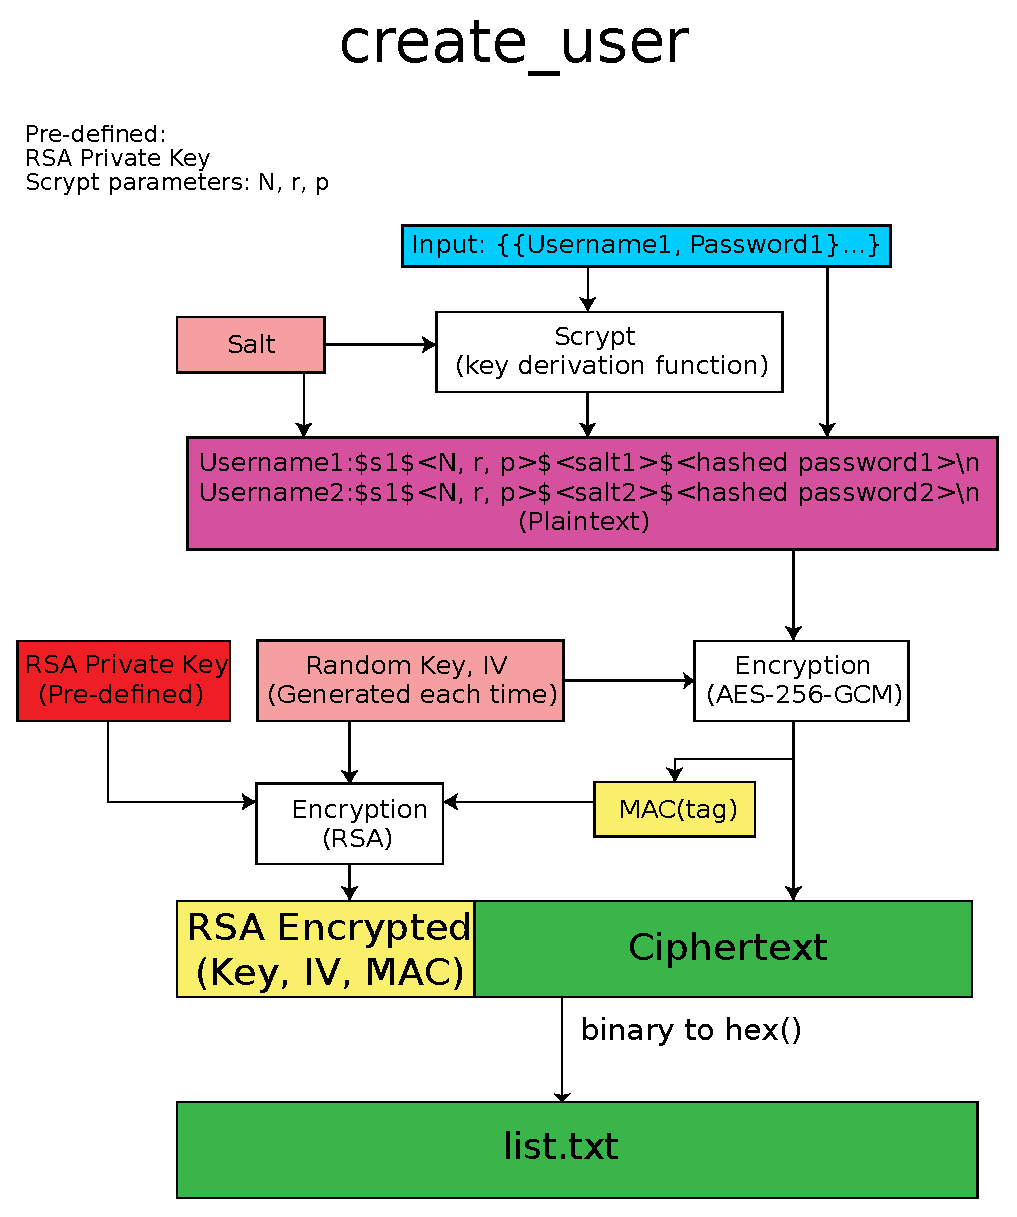
\includegraphics[width=\linewidth]{create.eps} 
\caption{Workflow of create\_user module}
\end{minipage}\hfill
\begin{minipage}{0.45\textwidth}
\centering
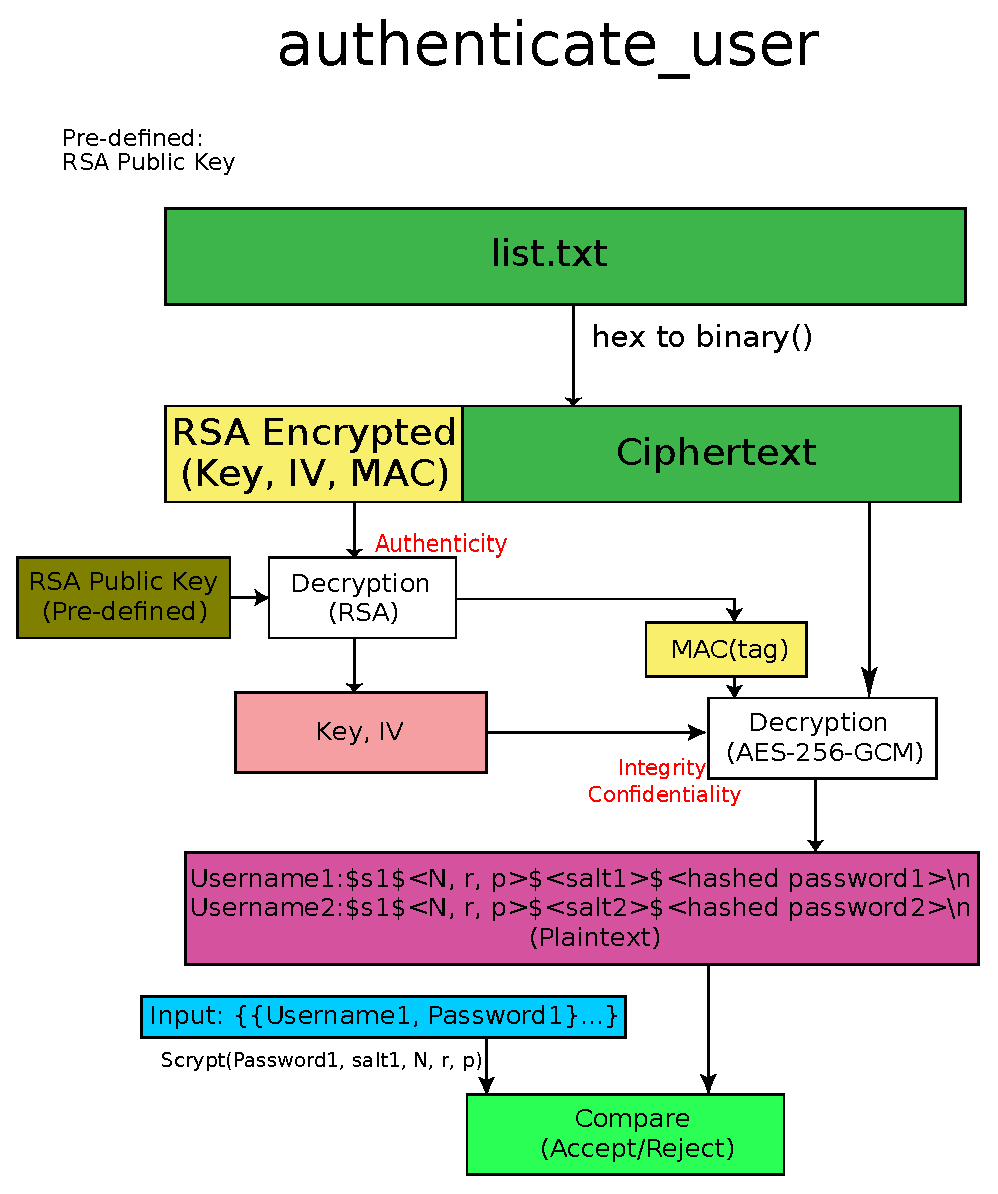
\includegraphics[width=\linewidth]{authenticate.eps}
\caption{Workflow of authenticate\_user module}
\end{minipage}
\end{figure}

Since the attack may be able to obtain the source code or use reverse engineering to attack the system, symmetric encryption won't help. In our design, we use RSA private key to encrypt the key, initialization vector and tag used by GCM encryption. The private key is stored in the secure \texttt{authenticate\_user} module. The public key is stored in \texttt{create\_user} module. The process is explained in the following two graph.Since the attack may be able to obtain the source code or use reverse engineering to attack the system, symmetric encryption won't help. In our design, we use RSA private key to encrypt the key, initialization vector and tag used by GCM encryption. The private key is stored in the secure \texttt{authenticate\_user} module. The public key is stored in \texttt{create\_user} module. The process is explained in the Fig. 1 and Fig. 2.

Our system are adopting a defense in depth approach, Table II summarized the protection features by our system.

\begin{table*}
\centering
\caption{Defense in depth}
\label{my-label}
\begin{tabular}{|l|l|l|l|l|}
\hline
\textbf{Attac\textbackslash Protect}                                                        & \textbf{\begin{tabular}[c]{@{}l@{}}Pw\\ hashing\end{tabular}}     & \textbf{\begin{tabular}[c]{@{}l@{}}RSA\\ Encryption\end{tabular}} & \textbf{AES GCM Encryption} & \textbf{Level of protection}                                                                                                                                                           \\ \hline
\textbf{Brute force}                                                           & Secure                                                            & Secure                                                            & Secure                      & \begin{tabular}[c]{@{}l@{}}Can protect weak password\\ since username are encrypted\end{tabular}                                                                                       \\ \hline
\textbf{\begin{tabular}[c]{@{}l@{}}Source code/\\ Reverse engine\end{tabular}} & Secure                                                            & \begin{tabular}[c]{@{}l@{}}Secure\\ (integrity)\end{tabular}      & Broken                      & \begin{tabular}[c]{@{}l@{}}list.txt is not modified, however\\ the username and hashed password\\ are known to attacker\end{tabular}                                                   \\ \hline
\textbf{\begin{tabular}[c]{@{}l@{}}Source code +\\ Brute force\end{tabular}}   & \begin{tabular}[c]{@{}l@{}}Rely on strong\\ password\end{tabular} & \begin{tabular}[c]{@{}l@{}}Secure\\ (integrity)\end{tabular}      & Broken                      & \begin{tabular}[c]{@{}l@{}}list.txt is not modified, howeverthe \\ username and hashed password are \\ known to attacker\\ User using strong password are still \\ secure\end{tabular} \\ \hline
\end{tabular}
\end{table*}


\ifCLASSOPTIONcaptionsoff
  \newpage
\fi


\begin{thebibliography}{1}
\bibitem{scrypt}
Colin Percival. Stronger Kye Derivation via Sequential Memory-hard Functions. \texttt{BSDCan'09}.

\bibitem{MCF}
Assurance Technologies. \emph{Modular Crypt Format}[Online]. 
Available: https://pythonhosted.org/passlib/modular\_crypt\_format.html

\bibitem{libscrypt}
libscrypt. \texttt{https://github.com/technion/libscrypt}

\bibitem{GCMNIST}
David A. McGrew and John Viega. The Galois/Counter Mode of Operation (GCM). \texttt{http://csrc.nist.gov/groups/ST/toolkit/BCM/documents /proposedmodes/gcm/gcm-spec.pdf}

%http://stackoverflow.com/questions/1220751/how-to-choose-an-aes-encryption-mode-cbc-ecb-ctr-ocb-cfb
%
%http://cseweb.ucsd.edu/~mihir/papers/oem.pdf
%
%http://crypto.stackexchange.com/questions/6842/how-to-choose-between-aes-ccm-and-aes-gcm-for-storage-volume-encryption
%
%http://hayageek.com/rsa-encryption-decryption-openssl-c/
%
%http://web.cs.ucdavis.edu/~rogaway/papers/modes.pdf
\end{thebibliography}



% that's all folks
\end{document}


